\section{Introduction}

\begin{frame}\frametitle{Motivation: How to create documents?}

\begin{itemize}
\item
  Types and distinctions

  \begin{itemize}
  \item
    Formal Documents: Journal articles, books, book chapters, theses,
    consulting reports, etc.
  \item
    Informal documents: preliminary analyses, statistical homework,
  \item
    Online content: web pages, blog posts, forum posts
  \item
    Browser metaphor versus page/slide-based metaphor
  \end{itemize}
\item
  Context

  \begin{itemize}
  \item
    When to use reproducible analysis?
  \item
    When to use knitr with R Markdown or LaTeX?
  \end{itemize}
\end{itemize}

\end{frame}

\begin{frame}\frametitle{What is \emph{reproducible analysis}?}

\begin{itemize}
\item
  Reproducibility varies on a continuum
\item
  One particular form:

  \begin{itemize}
  \item
    code transforms raw data and meta-data into processed data,
  \item
    code runs analyses on the data, and
  \item
    code incorporates analyses into a report
  \end{itemize}
\item
  Ideally, the process involves a one-click build
\item
  Public sharing of document, code, and data is optional, but forms part
  of gold standard of scientific openness
\item
  Goes by many names, particularly ``reproducible research'', but I
  prefer ``reproducible analysis''.
\end{itemize}

\tiny{
See also: \url{http://stats.stackexchange.com/a/15006/183} 
\url{https://github.com/jeromyanglim/rmarkdown-rmeetup-2012/issues/11}}

\end{frame}

\begin{frame}\frametitle{Aims of reproducible analysis}

\begin{itemize}
\item
  Ability to reproduce analysis
\item
  Increase accuracy

  \begin{itemize}
  \item
    Ability to verify analyses are consistent with intentions
  \item
    Ability to review analysis choices
  \end{itemize}
\item
  Increase clarity of communication
\item
  Increased trustworthiness

  \begin{itemize}
  \item
    Increased accuracy +
  \item
    Ability for others to verify
  \end{itemize}
\item
  Extensibility

  \begin{itemize}
  \item
    Ability to easily modify or re-use existing analyses
  \end{itemize}
\end{itemize}

\end{frame}

\begin{frame}\frametitle{Reproducible analysis in R}

\begin{block}{Typically:}

\begin{itemize}
\item
  Combine R and plain text file format to produce documents (e.g., pdfs,
  HTML documents, etc.)
\end{itemize}

\end{block}

\begin{block}{Popular Instances}

\begin{itemize}
\item
  Sweave
\item
  brew
\item
  knitr
\end{itemize}

\tiny{see also \url{http://cran.r-project.org/web/views/ReproducibleResearch.html}}

\end{block}

\end{frame}

\begin{frame}[fragile]\frametitle{Installation of software used in this
talk}

\begin{itemize}
\item
  R: \url{http://www.r-project.org/}
\item
  R Studio: \url{http://rstudio.org/}
\item
  In R:

  \begin{itemize}
  \item
    \texttt{install.packages("knitr)}
  \item
    \texttt{install.packages("markdown")}
  \item
    \texttt{install.packages("xtable")}
  \item
    \texttt{install.packages("ggplot2")}
  \item
    \texttt{install.packages("lattice")}
  \end{itemize}
\item
  pandoc:

  \begin{itemize}
  \item
    \url{http://johnmacfarlane.net/pandoc/}
  \end{itemize}
\item
  LaTeX distribution:

  \begin{itemize}
  \item
    E.g., TeXLive, MikTeX \url{http://www.latex-project.org/ftp.html}
  \end{itemize}
\end{itemize}

\end{frame}

\section{Markdown}

\begin{frame}\frametitle{What is markdown?}

\begin{itemize}
\item
  Simple, readable, intuitive, light-weight markup
\item
  Convert to HTML
\item
  Raw HTML can be interspersed to add functionality
\item
  Various extensions and flaours of markdown
\item
  Popular on websites: e.g., StackOverflow, GitHub, Reddit
\end{itemize}

\tiny{see also: \url{http://daringfireball.net/projects/markdown/ }}

\end{frame}

\begin{frame}\frametitle{Headings}

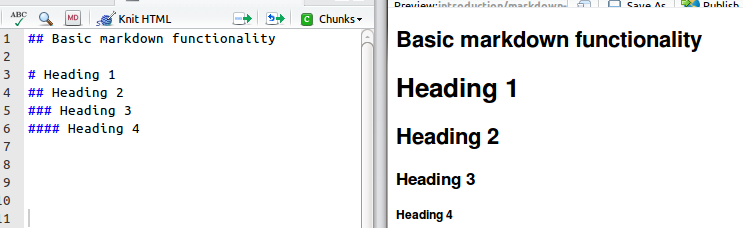
\includegraphics[width=4in]{figures/headings.png}

\end{frame}

\begin{frame}\frametitle{Basic formatting}

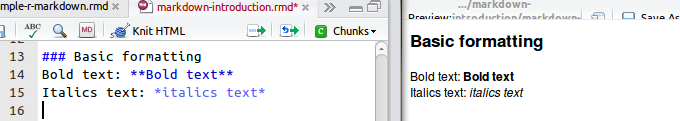
\includegraphics[width=4in]{figures/basic-formatting.png}

\end{frame}

\begin{frame}\frametitle{Paragraphs}

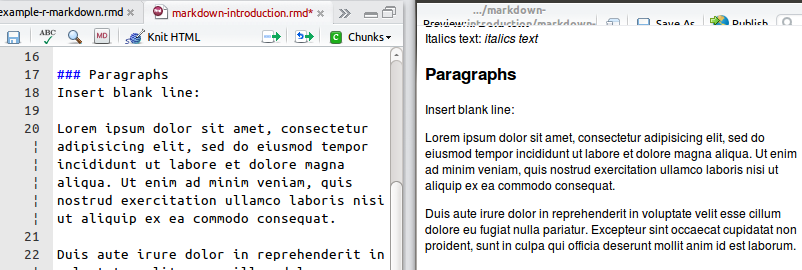
\includegraphics[width=4in]{figures/paragraphs.png}

\end{frame}

\begin{frame}\frametitle{Dot points}

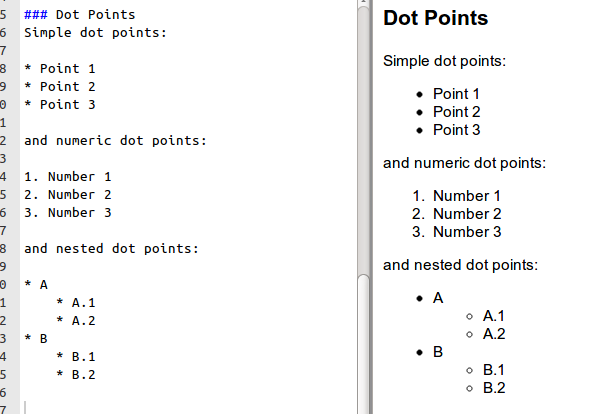
\includegraphics[width=4in]{figures/dot-points.png}

\end{frame}

\begin{frame}\frametitle{Equations}

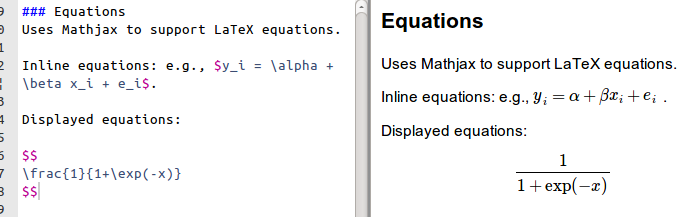
\includegraphics[width=4in]{figures/equations.png}

\begin{itemize}
\item
  Uses MathJaX to render LaTeX (and other) equations
\item
  Inserts MathJaX script reference into HTML header
\end{itemize}

\tiny{getting started: \url{http://jeromyanglim.blogspot.com.au/2010/10/getting-started-with-writing.html}}

\end{frame}

\begin{frame}\frametitle{Hyperlinks}


\includegraphics[width=4in]{figures/links.png}

\end{frame}

\begin{frame}\frametitle{Images}

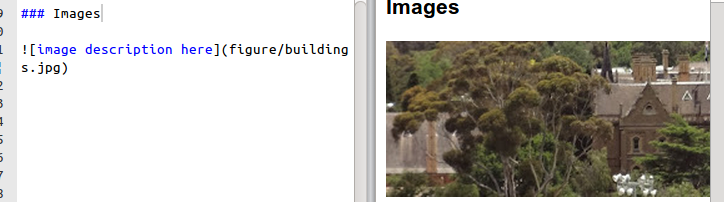
\includegraphics[width=4in]{figures/images.png}

\end{frame}

\begin{frame}\frametitle{Code}

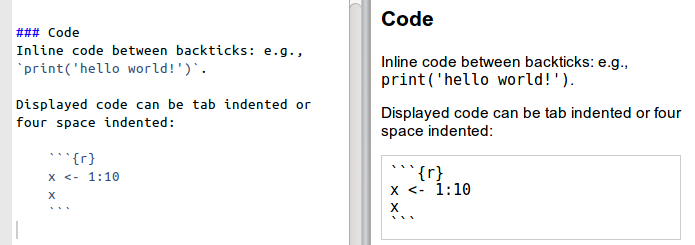
\includegraphics[width=4in]{figures/code.png}

\end{frame}

\begin{frame}\frametitle{Quotes}

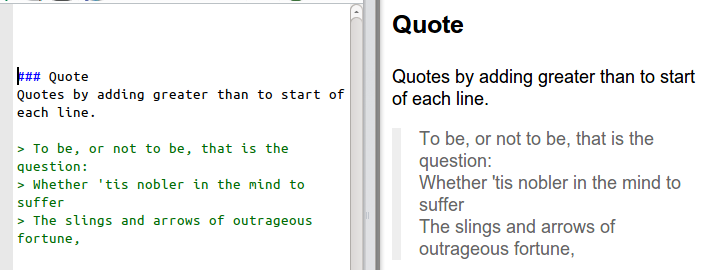
\includegraphics[width=4in]{figures/quote.png}

\end{frame}

\begin{frame}\frametitle{Tables}

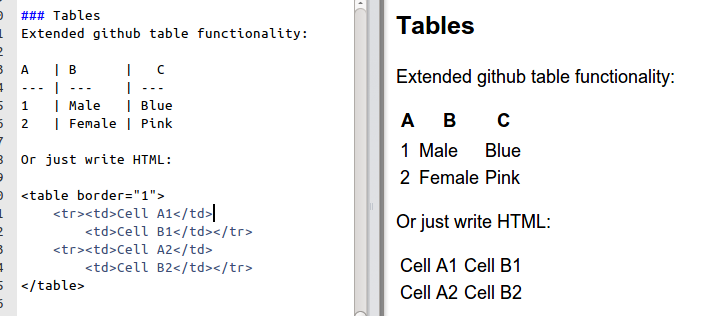
\includegraphics[width=4in]{figures/tables.png}

\end{frame}

\begin{frame}\frametitle{Raw HTML}

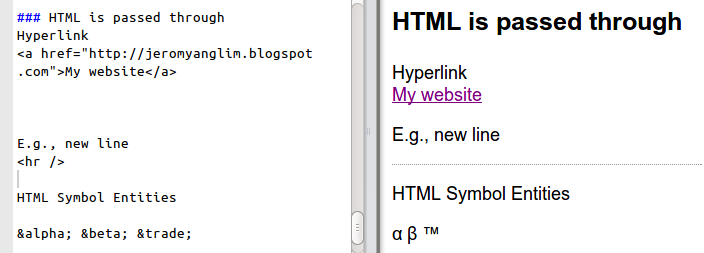
\includegraphics[width=4in]{figures/html.png}

\end{frame}

\section{knitr and R Markdown}

\begin{frame}\frametitle{knitr, R Markdown, and R Studio}

\begin{itemize}
\item
  knitr: R Package developed by Yihui Xie for weaving R (and other
  languages) with various markup languages
\item
  R Markdown: A file format that combines R code chunks and markdown
  text which is converted by knitr into markdown, and other formats
  (e.g., HTML, pdf, etc.).
\item
  R Studio: Open source, cross-platform IDE for R.
\end{itemize}

\end{frame}

\begin{frame}[fragile]\frametitle{Benefits of knitr}

\begin{itemize}
\item
  knitr supports many markups: LaTeX, Markdown, HTML, reStructuredText
\item
  knitr has really nice defaults
\item
  Tidy placement of generated files
\item
  Simplified figure production

  \begin{itemize}
  \item
    automatically print ggplot2 and lattice figures
  \item
    print figures by default
  \item
    permit interspersing of figures and console output
  \end{itemize}
\item
  Greater extensibility:

  \begin{itemize}
  \item
    output options
  \item
    supports languages other than R
  \end{itemize}
\item
  Simplified caching
\item
  And more: \url{http://yihui.name/slides/2012-knitr-RStudio.html}
\end{itemize}

\end{frame}

\begin{frame}\frametitle{Rstudio}

\begin{itemize}
\item
  Benefits of Rstudio as IDE for R

  \begin{itemize}
  \item
    Open source
  \item
    Works on Linux, Mac, and Windows
  \item
    Many useful features
  \item
    It just works
  \item
    Tight integration with knitr
  \end{itemize}
\item
  But many other options

  \begin{itemize}
  \item
    Emacs with ESS
  \item
    Vim with R plugin
  \item
    Eclipse with StatET
  \item
    etc.
  \end{itemize}
\end{itemize}

\end{frame}

\begin{frame}\frametitle{RMarkdown Examples}

\begin{itemize}
\item
  \emph{Introduction to R Markdown}
\item
  \emph{Statistics homework example}
\item
  \emph{Analysis of Winter Olympic Medals Example}
\end{itemize}

\end{frame}

\begin{frame}\frametitle{Rstudio screenshot}

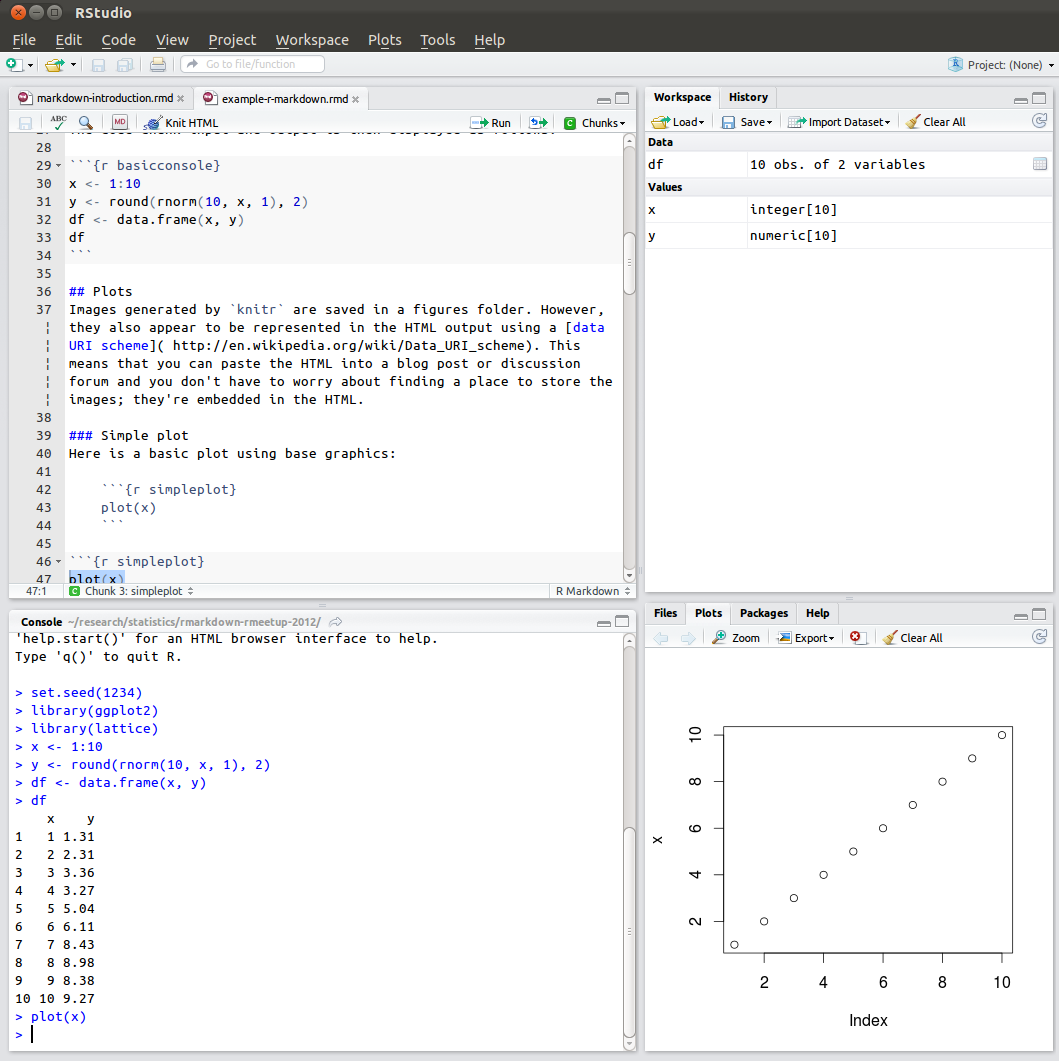
\includegraphics[width=3in]{figures/rstudio-screenshot.png}

\end{frame}

\begin{frame}[fragile]\frametitle{R Code chunks}

see http://yihui.name/knitr/options

\begin{verbatim}
```{r my_chunk_name, some_option='some_value'}
some_r_code
```
\end{verbatim}

\end{frame}

\begin{frame}[fragile]\frametitle{R Code chunks options}

\begin{block}{Global options:}

\begin{verbatim}
`r opts_chunk$set(opt = value)` # general form
`r opts_chunk$set(cache=TRUE)` # e.g, global cache
\end{verbatim}

\end{block}

\begin{block}{Some useful local options}

\begin{itemize}
\item
  Hide console input: \texttt{echo=FALSE}
\item
  Hide assorted messages:
  \texttt{warning=FALSE, error=FALSE, message=FALSE}
\item
  Hide console output: \texttt{results="hide"}
\item
  Display console input as is: \texttt{tidy=FALSE}
\item
  Output raw markup: \texttt{results="asis"}
\end{itemize}

\end{block}

\end{frame}

\begin{frame}[fragile]\frametitle{Inline R Code}

\begin{verbatim}
R Markdown     `r 2 + 2`       `r I(2+2)`
Markdown           `4`             4
HTML          <code>4</code>       4
\end{verbatim}

\end{frame}

\begin{frame}[fragile]\frametitle{Figures}

\begin{itemize}
\item
  Support for multiple figures in a code block

  \begin{itemize}
  \item
    also see e.g., \texttt{par(mfrow=c(2,2))} or \texttt{grid.arrange}
  \end{itemize}
\item
  Figures and console output can be interspersed in a code chunk
\item
  Various code chunk options

  \begin{itemize}
  \item
    see http://yihui.name/knitr/options
  \item
    \texttt{fig.width} and \texttt{fig.height}
  \item
    \texttt{dev} defaults to pdf for LaTeX and png for HTML/markdown
  \end{itemize}
\end{itemize}

\end{frame}

\begin{frame}[fragile]\frametitle{Tables}

\begin{itemize}
\item
  Many options for creating HTML Tables:

  \begin{itemize}
  \item
    R packages: \texttt{xtable}, \texttt{googleVis}, \texttt{R2HTML},
    \texttt{hwriter}
  \item
    markdown extentions: github, pandoc
  \item
    Custom R code
  \end{itemize}
\item
  \texttt{xtable} is a reasonable option
\item
  For informal reports just use console output
\item
  css can be added later to control table appearance
\item
  If you require sophisticated tables, you may want to switch to LaTeX
\end{itemize}

\end{frame}

\begin{frame}[fragile]\frametitle{\texttt{xtable} example}

\begin{verbatim}
print(xtable(my_data_frame, caption = "My Caption", 
    digits = 3), type = "html", 
    caption.placement = "top", 
    html.table.attributes = 
    "style=\"border: 1px solid black;\"")
\end{verbatim}

\centerline{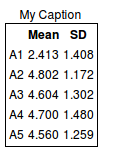
\includegraphics[height=1.5in]{figures/simple_table.png}}

\end{frame}

\begin{frame}[fragile]\frametitle{Caching}

Basic workflow:

\begin{itemize}
\item
  If knitting is quick, don't cache.
\item
  If knitting takes more than ten seconds add
  \texttt{\`}\texttt{r opts\_chunk\$set(cache=TRUE)}\texttt{\`} to the
  top of R Markdown file.
\item
  If caching is causing problems, delete contents of \texttt{cache}
  folder,
\item
  But if caching is causing problems and knitting takes a long time,
  name R code chunks and use the \texttt{dependson} option in knitr (see
  http://yihui.name/knitr/options). Naming also permits selective
  deletion of named R code chunks in the cache directory.
\end{itemize}

\end{frame}

\begin{frame}[fragile]\frametitle{R package: \texttt{markdown}}

\begin{itemize}
\item
  Maintained by Jeffrey Horner; Developed by devloped JJ Allaire,
  Jeffrey Horner, Vicent Marti, and Natacha Porte
\item
  R Package that creates more options for converting Markdown to HTML
\item
  \texttt{markdownToHTML("file.md", "file.html", options=c(...))}
\item
  The default options are
  \texttt{"hard\_wrap", "use\_xhml", "smartypants", "base64\_images"}
\end{itemize}

\end{frame}

\begin{frame}[fragile]\frametitle{Replicating R Studio's
\texttt{Knit to HTML}}

\begin{verbatim}
require(knitr) # for knitting from rmd to md
require(markdown) # for md to html 
knit('test.rmd', 'test.md') # creates md 
markdownToHTML('test.md', 'test.html') # create html
browseURL(paste('file://', 
    file.path(getwd(),'test.html'), 
    sep='')) # open file in browser
\end{verbatim}

see \texttt{?markdownHTMLOptions} for more options. E.g.,

\begin{verbatim}
markdownToHTML('test.md', 'test.html', 
    options='fragment_only')
\end{verbatim}

\end{frame}

\begin{frame}[fragile]\frametitle{pandoc}

\begin{itemize}
\item
  pandoc is a library and command-line tool for converting between many
  document formats (e.g., HTML, markdown, pdf, LaTeX, docx; also
  supports multiple plain text slide formats such as beamer)
\item
  Lots of options
\item
  Often requires thought in order to minimise conversion issues
\end{itemize}

\begin{block}{Example}

\begin{verbatim}
pandoc -s file.html -o file.pdf
\end{verbatim}

\end{block}

\end{frame}

\begin{frame}[fragile]\frametitle{One-click build}

\begin{itemize}
\item
  For simple documents, click \texttt{knit to HTML} in RStudio
\item
  For complex documents use a command-line option:

  \begin{itemize}
  \item
    e.g., \texttt{makefile}, \texttt{Rscript}, etc.
  \item
    combine with \texttt{pandoc}, \texttt{knitr} options,
    \texttt{markdown} options, text manipulation tools (e.g., sed, awk,
    scripting languages) etc. to flexibly produce a varity of documents
  \end{itemize}
\end{itemize}

\end{frame}

\section{LaTeX}

\begin{frame}\frametitle{Example of LaTeX}

\emph{If time permits, show example of knitr with LaTeX}

\end{frame}

\section{Conclusion}

\begin{frame}\frametitle{Final thoughts}

\begin{itemize}
\item
  knitr and R Markdown

  \begin{itemize}
  \item
    It makes reproducible analysis as simple as one click
  \item
    Great tool for:

    \begin{itemize}
    \item
      quick analyses for self and colleagues
    \item
      doing homework
    \item
      creating teaching resources
    \item
      blog posts, websites, etc.
    \end{itemize}
  \item
    Scope to make more complex documents, but at a certain point it may
    be worth exploring other tools
  \end{itemize}
\item
  knitr and R LaTeX

  \begin{itemize}
  \item
    Great for journal articles, theses, books (e.g., citations,
    cross-references, printed works, equations)
  \end{itemize}
\item
  As your needs get more complex

  \begin{itemize}
  \item
    pandoc, makefiles, knitr options, markdown package options, scripts,
    etc.
  \end{itemize}
\end{itemize}

\end{frame}

\begin{frame}[fragile]\frametitle{Links}

\begin{itemize}
\item
  knitr: \url{http://yihui.name/knitr/}
\item
  R Studio: \url{http://rstudio.org/}
\item
  R Markdown with R Studio:
  \url{http://rstudio.org/docs/authoring/using_markdown}
\item
  My Posts
  \url{http://jeromyanglim.blogspot.com.au/search/label/reproducible%20research}
\end{itemize}

\begin{block}{Places to ask questions}

\begin{itemize}
\item
  R on StackOverflow: \url{http://stackoverflow.com/questions/tagged/r}
\item
  LaTeX: \url{http://tex.stackexchange.com/}
\item
  knitr: \url{https://github.com/yihui/knitr/issues}
\end{itemize}

\end{block}

\end{frame}

\begin{frame}\frametitle{Thank You}

\begin{center}
\LARGE{Questions?}
\end{center}

\end{frame}
